\documentclass{standalone}
\usepackage{tikz}
\usetikzlibrary{patterns, positioning}


\begin{document}
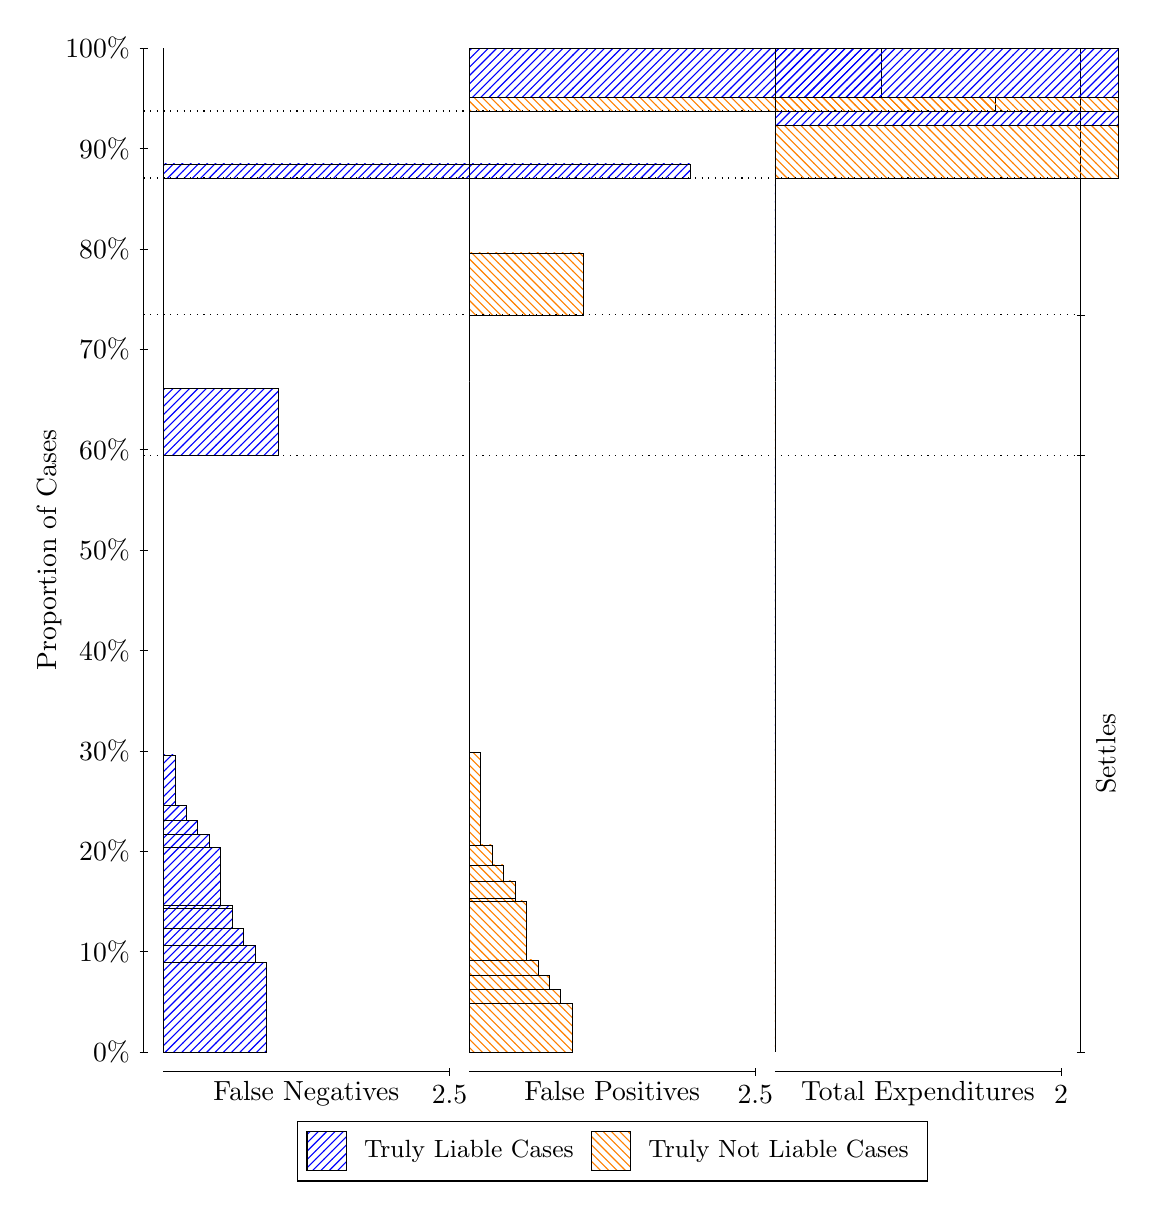
\begin{tikzpicture}
\draw[black, very thin] (1.5,1.75) -- (1.5,14.5);
\node[rotate=90, text=black, anchor=center] at (0.3, 8.125) {Proportion of Cases};
\draw[black, very thin] (1.45,1.75) -- (1.55,1.75);
\node[text=black, anchor=east] at (1.45, 1.75) {0\%};
\draw[black, very thin] (1.45,3.025) -- (1.55,3.025);
\node[text=black, anchor=east] at (1.45, 3.025) {10\%};
\draw[black, very thin] (1.45,4.3) -- (1.55,4.3);
\node[text=black, anchor=east] at (1.45, 4.3) {20\%};
\draw[black, very thin] (1.45,5.575) -- (1.55,5.575);
\node[text=black, anchor=east] at (1.45, 5.575) {30\%};
\draw[black, very thin] (1.45,6.85) -- (1.55,6.85);
\node[text=black, anchor=east] at (1.45, 6.85) {40\%};
\draw[black, very thin] (1.45,8.125) -- (1.55,8.125);
\node[text=black, anchor=east] at (1.45, 8.125) {50\%};
\draw[black, very thin] (1.45,9.4) -- (1.55,9.4);
\node[text=black, anchor=east] at (1.45, 9.4) {60\%};
\draw[black, very thin] (1.45,10.675) -- (1.55,10.675);
\node[text=black, anchor=east] at (1.45, 10.675) {70\%};
\draw[black, very thin] (1.45,11.95) -- (1.55,11.95);
\node[text=black, anchor=east] at (1.45, 11.95) {80\%};
\draw[black, very thin] (1.45,13.225) -- (1.55,13.225);
\node[text=black, anchor=east] at (1.45, 13.225) {90\%};
\draw[black, very thin] (1.45,14.5) -- (1.55,14.5);
\node[text=black, anchor=east] at (1.45, 14.5) {100\%};

\draw[black, very thin] (13.4,1.75) -- (13.4,14.5);
\draw[black, very thin] (13.35,1.75) -- (13.45,1.75);
\node[anchor=west] at (13.35, 1.75) {};
\draw[black, very thin] (13.35,9.3232) -- (13.45,9.3232);
\node[anchor=west] at (13.35, 9.3232) {};
\draw[black, very thin] (13.35,11.112) -- (13.45,11.112);
\node[anchor=west] at (13.35, 11.112) {};
\draw[black, very thin] (13.35,12.849) -- (13.45,12.849);
\node[anchor=west] at (13.35, 12.849) {};
\draw[black, very thin] (13.35,13.7) -- (13.45,13.7);
\node[anchor=west] at (13.35, 13.7) {};
\draw[black, very thin] (13.35,14.5) -- (13.45,14.5);
\node[anchor=west] at (13.35, 14.5) {};

\draw[black, very thin, pattern color=blue, pattern=north east lines] (1.75,1.75) rectangle (3.058,2.8895);
\draw[black, very thin, pattern color=blue, pattern=north east lines] (1.75,2.8895) rectangle (2.9127,3.1081);
\draw[black, very thin, pattern color=blue, pattern=north east lines] (1.75,3.1081) rectangle (2.7673,3.3156);
\draw[black, very thin, pattern color=blue, pattern=north east lines] (1.75,3.3156) rectangle (2.622,3.5762);
\draw[black, very thin, pattern color=blue, pattern=north east lines] (1.75,3.5762) rectangle (2.622,3.6084);
\draw[black, very thin, pattern color=blue, pattern=north east lines] (1.75,3.6084) rectangle (2.4767,4.3447);
\draw[black, very thin, pattern color=blue, pattern=north east lines] (1.75,4.3447) rectangle (2.3313,4.5155);
\draw[black, very thin, pattern color=blue, pattern=north east lines] (1.75,4.5155) rectangle (2.186,4.695);
\draw[black, very thin, pattern color=blue, pattern=north east lines] (1.75,4.695) rectangle (2.0407,4.8863);
\draw[black, very thin, pattern color=blue, pattern=north east lines] (1.75,4.8863) rectangle (1.8953,5.5232);
\draw[black, very thin, pattern color=orange, pattern=north west lines] (1.75,5.5232) rectangle (1.75,9.3232);
\draw[black, very thin, pattern color=blue, pattern=north east lines] (1.75,9.3232) rectangle (3.2033,10.173);
\draw[black, very thin, pattern color=orange, pattern=north west lines] (1.75,10.173) rectangle (1.75,11.112);
\draw[black, very thin, pattern color=orange, pattern=north west lines] (1.75,11.112) rectangle (1.75,11.898);
\draw[black, very thin, pattern color=blue, pattern=north east lines] (1.75,11.898) rectangle (1.75,12.849);
\draw[black, very thin, pattern color=blue, pattern=north east lines] (1.75,12.849) rectangle (8.4353,13.028);
\draw[black, very thin, pattern color=orange, pattern=north west lines] (1.75,13.028) rectangle (1.75,13.7);
\draw[black, very thin, pattern color=orange, pattern=north west lines] (1.75,13.7) rectangle (1.75,13.878);
\draw[black, very thin, pattern color=blue, pattern=north east lines] (1.75,13.878) rectangle (1.75,14.5);
\draw[black, very thin, pattern color=orange, pattern=north west lines] (5.6333,1.75) rectangle (6.9413,2.3622);
\draw[black, very thin, pattern color=orange, pattern=north west lines] (5.6333,2.3622) rectangle (6.796,2.5461);
\draw[black, very thin, pattern color=orange, pattern=north west lines] (5.6333,2.5461) rectangle (6.6507,2.7255);
\draw[black, very thin, pattern color=orange, pattern=north west lines] (5.6333,2.7255) rectangle (6.5053,2.9196);
\draw[black, very thin, pattern color=orange, pattern=north west lines] (5.6333,2.9196) rectangle (6.36,3.6697);
\draw[black, very thin, pattern color=orange, pattern=north west lines] (5.6333,3.6697) rectangle (6.2147,3.7031);
\draw[black, very thin, pattern color=orange, pattern=north west lines] (5.6333,3.7031) rectangle (6.2147,3.9218);
\draw[black, very thin, pattern color=orange, pattern=north west lines] (5.6333,3.9218) rectangle (6.0693,4.1259);
\draw[black, very thin, pattern color=orange, pattern=north west lines] (5.6333,4.1259) rectangle (5.924,4.3802);
\draw[black, very thin, pattern color=orange, pattern=north west lines] (5.6333,4.3802) rectangle (5.7787,5.5501);
\draw[black, very thin, pattern color=blue, pattern=north east lines] (5.6333,5.5501) rectangle (5.6333,9.3232);
\draw[black, very thin, pattern color=orange, pattern=north west lines] (5.6333,9.3232) rectangle (5.6333,10.262);
\draw[black, very thin, pattern color=blue, pattern=north east lines] (5.6333,10.262) rectangle (5.6333,11.112);
\draw[black, very thin, pattern color=orange, pattern=north west lines] (5.6333,11.112) rectangle (7.0867,11.898);
\draw[black, very thin, pattern color=blue, pattern=north east lines] (5.6333,11.898) rectangle (5.6333,12.849);
\draw[black, very thin, pattern color=orange, pattern=north west lines] (5.6333,12.849) rectangle (5.6333,13.521);
\draw[black, very thin, pattern color=blue, pattern=north east lines] (5.6333,13.521) rectangle (5.6333,13.7);
\draw[black, very thin, pattern color=orange, pattern=north west lines] (5.6333,13.7) rectangle (12.319,13.878);
\draw[black, very thin, pattern color=blue, pattern=north east lines] (5.6333,13.878) rectangle (10.865,14.5);
\draw[black, very thin, pattern color=orange, pattern=north west lines] (9.5167,1.75) rectangle (9.5167,5.5501);
\draw[black, very thin, pattern color=blue, pattern=north east lines] (9.5167,5.5501) rectangle (9.5167,9.3232);
\draw[black, very thin, pattern color=orange, pattern=north west lines] (9.5167,9.3232) rectangle (9.5167,10.262);
\draw[black, very thin, pattern color=blue, pattern=north east lines] (9.5167,10.262) rectangle (9.5167,11.112);
\draw[black, very thin, pattern color=orange, pattern=north west lines] (9.5167,11.112) rectangle (9.5167,11.898);
\draw[black, very thin, pattern color=blue, pattern=north east lines] (9.5167,11.898) rectangle (9.5167,12.849);
\draw[black, very thin, pattern color=orange, pattern=north west lines] (9.5167,12.849) rectangle (13.877,13.521);
\draw[black, very thin, pattern color=blue, pattern=north east lines] (9.5167,13.521) rectangle (13.877,13.7);
\draw[black, very thin, pattern color=orange, pattern=north west lines] (9.5167,13.7) rectangle (13.877,13.878);
\draw[black, very thin, pattern color=blue, pattern=north east lines] (9.5167,13.878) rectangle (13.877,14.5);
\draw[black, dotted] (1.5,9.3232) -- (13.4,9.3232);
\draw[black, dotted] (1.5,11.112) -- (13.4,11.112);
\draw[black, dotted] (1.5,12.849) -- (13.4,12.849);
\draw[black, dotted] (1.5,13.7) -- (13.4,13.7);
\draw[black, very thin] (1.75,1.5) -- (5.3833,1.5);
\node[text=black, anchor=north] at (3.5667, 1.5) {False Negatives};
\draw[black, very thin] (5.3833,1.45) -- (5.3833,1.55);
\node[text=black, anchor=north] at (5.3833, 1.45) {2.5};

\draw[black, very thin] (5.6333,1.5) -- (9.2667,1.5);
\node[text=black, anchor=north] at (7.45, 1.5) {False Positives};
\draw[black, very thin] (9.2667,1.45) -- (9.2667,1.55);
\node[text=black, anchor=north] at (9.2667, 1.45) {2.5};

\draw[black, very thin] (9.5167,1.5) -- (13.15,1.5);
\node[text=black, anchor=north] at (11.333, 1.5) {Total Expenditures};
\draw[black, very thin] (13.15,1.45) -- (13.15,1.55);
\node[text=black, anchor=north] at (13.15, 1.45) {2};

\node[text=black, centered, rotate=90] at (13.72, 5.5366) {Settles};





\draw (7.449999999999999,1.5) node[draw=none] (baseCoordinate) {};
\begin{scope}[align=center]
        \matrix[scale=0.5, draw=black, below=0.5cm of baseCoordinate, nodes={draw}, column sep=0.1cm]{
            \node[rectangle, draw, minimum width=0.5cm, minimum height=0.5cm, pattern color=blue, pattern=north east lines] {}; &
            \node[draw=none, font=\small, text=black] (B) {Truly Liable Cases}; &
            \node[rectangle, draw, minimum width=0.5cm, minimum height=0.5cm, pattern color=orange, pattern=north west lines] {}; &
            \node[draw=none, font=\small, text=black] (B) {Truly Not Liable Cases}; \\
            };
\end{scope}

\end{tikzpicture}
\end{document}